\documentclass{article}
\usepackage{graphicx}
\usepackage{wrapfig}
\graphicspath{{./images/}}

\author{Hawley, Adam}
\title{Lecture 3: Photometric Image Formation\\Part 1}
\begin{document}
\maketitle
\tableofcontents
\newpage

\section{Types of Sensor}
There are many different types of sensors used in computer vision:
\begin{itemize}
	\item Optical
	\begin{itemize} \item CCD, Photodiodes, Photomultipliers \end{itemize}
	\item Infra-red (thermal imaging cameras)
	\begin{itemize} \item CCD (Cooled), Photodiodes \end{itemize}
	\item Synthetic Aperture Radaaar (SAR)
	\begin{itemize} \item Radar, Antenna \end{itemize}
	\item Range Sensors
	\begin{itemize} \item Laser \& Photodiode \end{itemize}
	\item MRI
	\begin{itemize} \item Magnetic field gradients applied causing production of rotating magnetic field which can be measured. \end{itemize}
	\item PET/CAT
	\begin{itemize} \item Simulated radiation emission via magnetic field or radio isotope. \end{itemize}
\end{itemize}
\section{From Light to Images}
\subsection{Definitions}
\begin{itemize}
	\item {\textit{\textbf {Irradiance}}}: power incident on a surface (power per unit area).
	\item {\textit{\textbf {Radiance}}}: power travelling from a source (power per unit solid angle per unit projected source area).
\end{itemize}
\subsection{Charge-Coupled Devices}
The most common devixe for digitising image information is a charge-coupled device (CCD). 
They are made up of a square array of solid-state capacitors: \\
\begin{figure}[htbp]
	\centering
	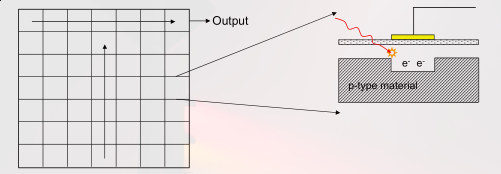
\includegraphics[width=0.9\textwidth]{ccd.png}
	\caption{The flow of electrons inside a CCD}
	\label{fig:CCD}
\end{figure} \\
From the photo-electric effect photons of light knock out electrons from the upper plate and hence charge accumulates in the electron capture ``{\it wells}".
Using a shift register, capacitors tranfer their contents to the appropriate neighbour.
The final capacitor dumps the charge for each capacitor into the analogue-digital converter (ADC).
The dump happens once for each capacitor until the contents of each one has been read. \\
\begin{figure}
	\centering
	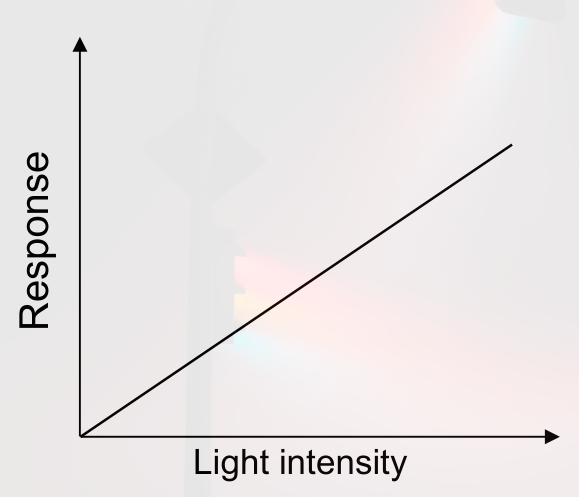
\includegraphics[width=0.3\textwidth]{ccdResponse1.png}
	\caption{Ideal response of a CCD}
	\label{fig:ccdResponse1}
\end{figure}
\\
The ideal reading from a CCD would be as simple as ``$output = gain\cdot input$". See figure \ref{fig:ccdResponse1}.
\begin{figure}
	\centering
	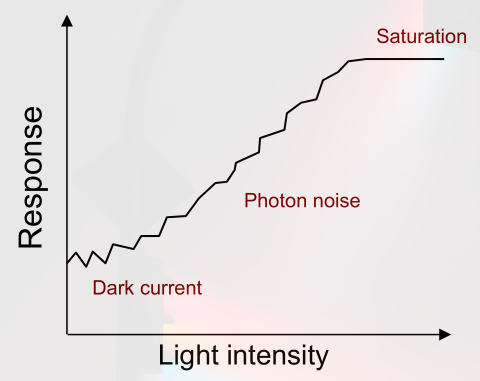
\includegraphics[width=0.4\textwidth]{ccdResponse2.png}
	\caption{Typical response of a CCD}
	\label{fig:ccdResponse2}
\end{figure}
However, a typical reading from a CCD also includes bias and noise (as can be seen in \ref{fig:ccdResponse2}.
(``$output = gain \cdot input + bias + noise$'')
The noise mostly comes from the following sources:
\begin{itemize}
	\item Dark Cuttent - Thermal noise.
	\item Photon Noise - Quantum noise.
	\item Quantisation of pixels.
	\item Amplifier
\end{itemize}
\newpage
\section{Saturation}
The electron capture wells inside the CCD have a finite capacity $\approx 700 \epsilon ^-/\mu m^2$.
That means that there is roughly a maximum of 100,000 $e^-$ per well in a typicall CCD.
When a well is full, the pixel is said to be saturated.
CCDs have a small illumination range (this is what {\it HDR imaging} attempts to overcome).
In an 8-bit image, a pixel brightness of 255 indicates saturation.
\section{Noise}
\subsection{Signal to Noise Ratio}
The level of noise relative to the signal strength is measured by the {\it signal to noise ratio}. This is often expressed in Decibels (10 times the logarithm of the ratio):

\centerline{$SNR (dB) = 10\log _{10}\frac{signal power}{noise power}$}

10dB is a tenfold increase in power, 3dB is a doubling of signal power.

\subsection{Photon Noise (Shot noise)}
\begin{itemize}
	\item Light sources emit light in photons.
		\begin{itemize}
			\item $\beta$ photons/second on average 
			\item However the photons are emitted randomly.
		\end{itemize}
	\item They follow a Poisson distribution of time t.
		\begin{itemize}
			\item Therefore there is a mean intensity of $\mu = \beta t$
			\item And a standard deviation of $\sigma = \sqrt{\beta t}$
		\end{itemize}
\end{itemize}
Note: At mid-brightness levels the {\it Signal to Noise Ratio}(SNR) for photon noise is around 23dB.
\subsection{Dark Current}
{\it Dark Current} is a product of thermal energy from within the CCD.
Electrons are displaced over time that are independant of light actually falling on the sensor (therefore this effect builds up with exposure).
The effect also obviously increases at higher environmental temperatures.
The manufacturing process means certain electron wells may have higher than average dark current ({\it hot pixels}).
{\it Dark fram subtraction} can be used to remove an estimate of the mean pattern of dark current.
However, dark current is also random and hence why it still affects CCD readings.
The randomness of the dark current follows the Poisson distribution just as the photon noise did.

Dark current can be easily shown by taking a picture in complete darkness and inspecting the images to see that it is unlikely that all the pixels will be of absolute darkness.

The SNR for dark current in mid-light levels is approximately 38dB.
\subsection{Quantisation noise}
Pixels in photos are digitised to $2^B$ levels. There is a uniformly distributed error on values of $\pm\frac{1}{2}$. This distribution leads to the following properties:
\begin{itemize}
	\item Mean: $\mu = 0$
	\item Standard Deviation: $\sigma =\frac{1}{\sqrt{12}}$ 
	\item $SNR = 10log_{10}(2^{B-1}\cdot \sqrt{12})$
\end{itemize}

$SNR = 26dB$ for 8-bit digitisation, which is better than  the photon noise ratio. Photon noise is the limiting factor of CCDs.
\section{CCDs and Colour}
CCDs record photons of all wavelengths, hence they are all monochrome.
A colour image requires red, green and blue values.

To get colour when using a CCD, there are three options:
\begin{enumerate}
	\item Take 3 separate images with a different filter places over the lens. This technique can use filters to allow other frequencies to pass and is hence a multispectral camera. However this method can have issues with motion between frames.
	\item Use a beamsplitter and 3 different CCDs, each with their own colour filter. Using the beamsplitter means that one can have instantaneous colour image capture but careful calibration is required to get exact correspondence between pixels of 3 cameras and it is 3 times more expensive.
	\item Place filters over individual pixels in a mosaic pattern. This is the most common approach. 
		There are more green than red/blue filters since human vision has higher resolution in green than in red/blue. 
		The colours must be interpolated (the process of {\it demosaicing}).
		This method also reduces the effective resolution of the CCD.
\end{enumerate}
\end{document}
